%%%%%%%%%%%%%%%%%%%%%%%%%%%%%%%%%%%%%%%%%
% University/School Laboratory Report
% LaTeX Template
% Version 3.1 (25/3/14)
%
% This template has been downloaded from:
% http://www.LaTeXTemplates.com
%
% Original author:
% Linux and Unix Users Group at Virginia Tech Wiki 
% (https://vtluug.org/wiki/Example_LaTeX_chem_lab_report)
%
% License:
% CC BY-NC-SA 3.0 (http://creativecommons.org/licenses/by-nc-sa/3.0/)
%
%%%%%%%%%%%%%%%%%%%%%%%%%%%%%%%%%%%%%%%%%

%----------------------------------------------------------------------------------------
%	PACKAGES AND DOCUMENT CONFIGURATIONS
%----------------------------------------------------------------------------------------

\documentclass[12pt]{article}

%\usepackage[version=3]{mhchem} % Package for chemical equation typesetting
%\usepackage{siunitx} % Provides the \SI{}{} and \si{} command for typesetting SI units
\usepackage[left=1in,top=1in,right=1in,bottom=1in]{geometry} % Document margins
\usepackage{graphicx} % Required for the inclusion of images
\usepackage{pdfpages}
\usepackage{natbib} % Required to change bibliography style to APA
\usepackage{amsmath} % Required for some math elements 

\setlength\parindent{0pt} % Removes all indentation from paragraphs

\renewcommand{\labelenumi}{\alph{enumi}.} % Make numbering in the enumerate environment by letter rather than number (e.g. section 6)

%\usepackage{times} % Uncomment to use the Times New Roman font

%----------------------------------------------------------------------------------------
%	DOCUMENT INFORMATION
%----------------------------------------------------------------------------------------

\title{\textbf{Find A Room} \\ Project Backlog \\ CS 307} % Title

\author{Team \textsc{13}(Snoxy)} % Author name

\date{\today} % Date for the report

\begin{document}

\maketitle % Insert the title, author and date

\begin{center}
\begin{tabular}{l r}
Members: & Nathan Chang \\ % Partner names
& Xiaojing Ji \\
& Zilun Mai(Owen) \\
& Saranyu Phusit(Gott) \\
& Yao Xiao \\
\\
\bigskip
Instructor: & Professor Buster Dunsmore \\% Instructor/supervisor 
Project Coordinator: & Miguel Villarreal-Vasquez % Instructor/supervisor

\end{tabular}
\end{center}

% If you wish to include an abstract, uncomment the lines below
% \begin{abstract}
% Abstract text
% \end{abstract}

%----------------------------------------------------------------------------------------
%	SECTION 1
%----------------------------------------------------------------------------------------


\newpage
\section{Problem Statement}

Every year, new students and visitors have trouble finding restrooms, water fountains, classrooms, etc. We are going to write a mobile application that will give directions indoors by scanning QR codes put on walls throughout a building. The app will direct them towards their destination from where they are.


\section{Background Information}

When we went to the first CS30700 class, we all had to explore a new building, Lynn hall. It took everyone a while to find out how to get to this classroom with all the twists and turns that Lynn has. Because of the confusing layout, we thought that if we could get directions to the classroom with our mobile device, we would save time and confusion. We are planning to design a mobile app targeting students at Purdue university who are either new to the campus or unfamiliar with some of the buildings. This application will help these students find their classrooms or rest rooms until they are used to getting to their destination without the aid of this application. While this program will provide directions and maps like a google map, we plan on making it work without a connection to the internet. However GPS can’t provide the navigation that requires higher accuracy, so GPS can not satisfy user needs. There is an indoor navigation system on the market called WifiSLAM which Apple is spending \$20 million to buy it. It requires wifi installation on the floor and it is too expensive. We will do this by having all the map data stored in the app as a graph with nodes marking special locations on each floor. The reason for not using the internet is because sometimes in the lower floors, the internet services are slow beyond belief. In order to get our location, we will have QR codes placed around the floors which can be scanned to locate you with more precision than a GPS can provide. One limitation that we will face is getting all the map data even if there is a provided map on the floor. We can use measurements of hallways to draw a map for ourselves is there is no provided map on the floor.


\section{Requirements}
After grabbing the background information, our team decides to design a mobile application which is able to offer precise navigation. In order to know more details of users’ need and where needs to be designed carefully before build up our application better, we apply a list to show all functional and nonfunctional requirements.
\begin{center}
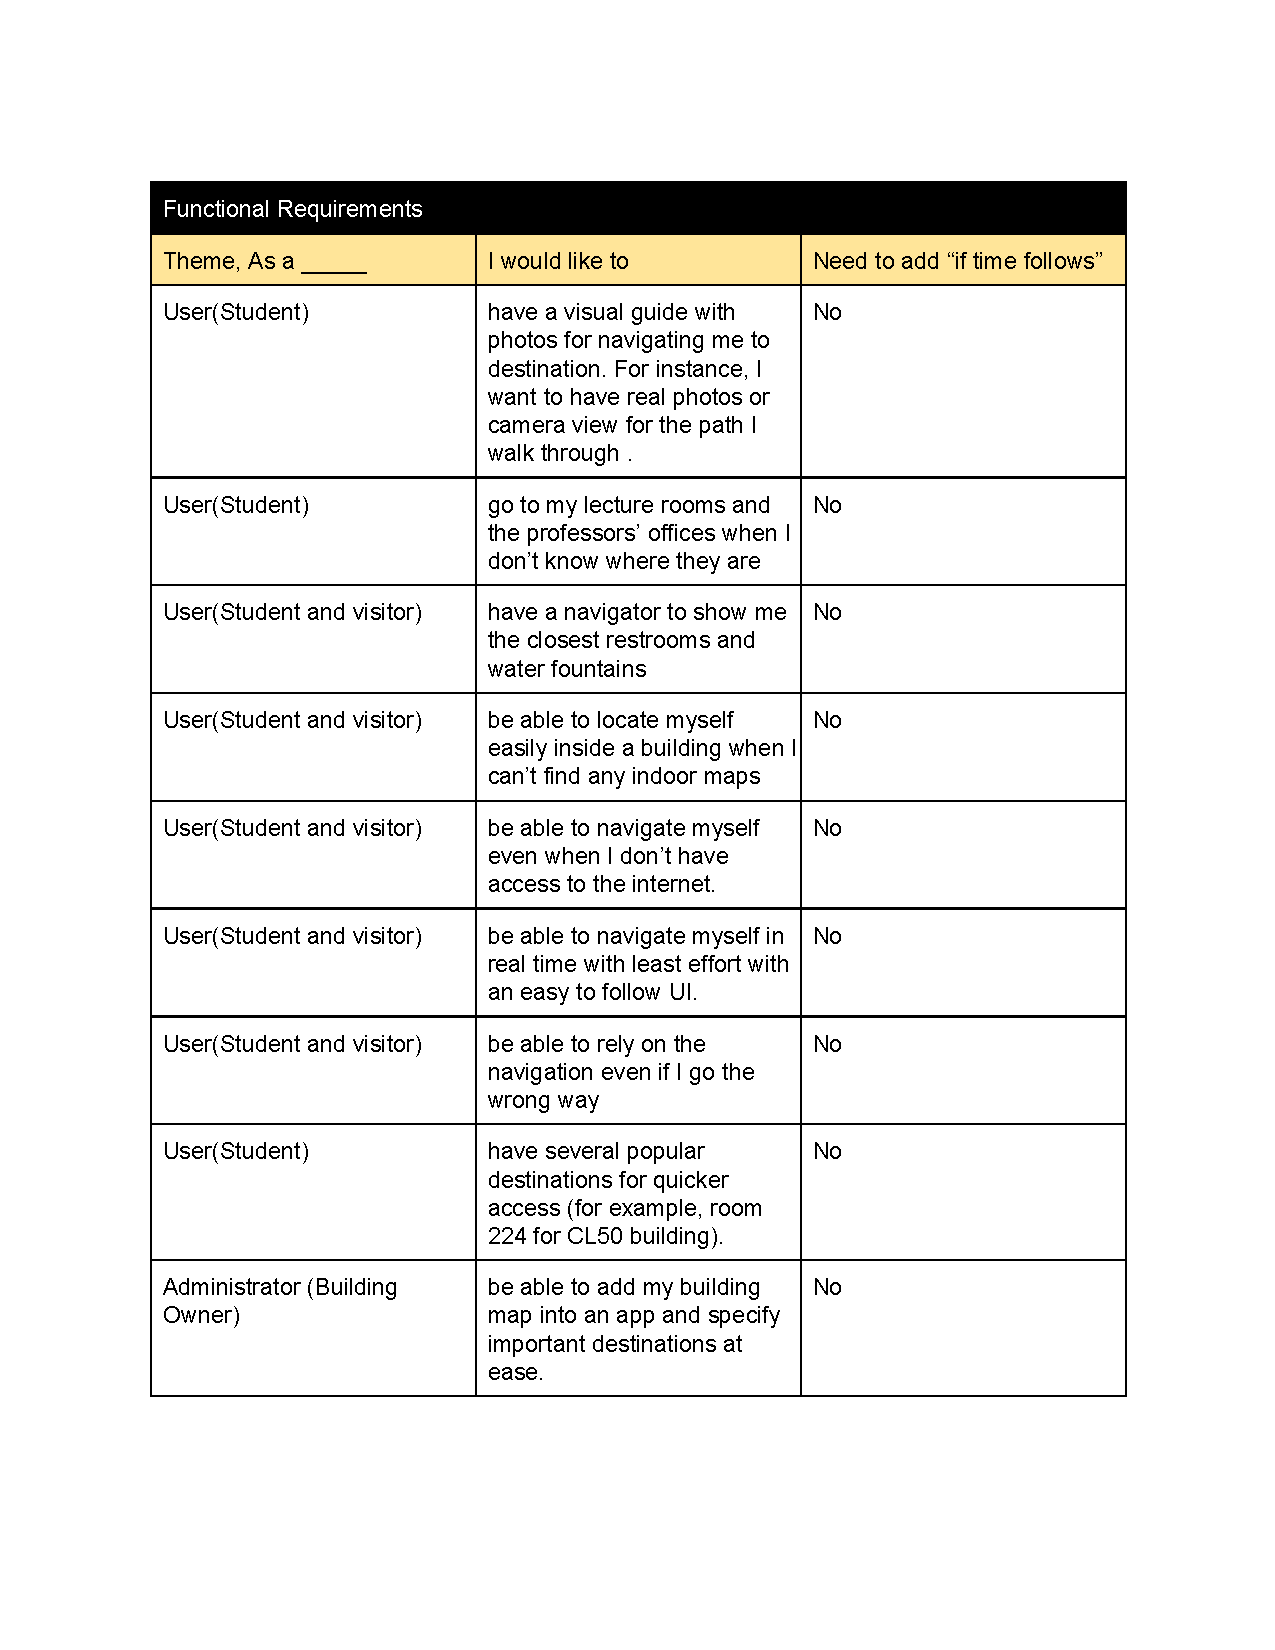
\includepdf[pages={1,2}]{requirement.pdf}
\end{center}

\end{document}